\documentclass{beamer}
\usepackage[utf8]{inputenc}

\usetheme{Madrid}
\usecolortheme{default}
\usepackage{amsmath,amssymb,amsfonts,amsthm}
\usepackage{txfonts}
\usepackage{tkz-euclide}
\usepackage{listings}
\usepackage{adjustbox}
\usepackage{array}
\usepackage{tabularx}
\usepackage{gvv}
\usepackage{lmodern}
\usepackage{circuitikz}
\usepackage{tikz}
\usepackage{graphicx}

\setbeamertemplate{page number in head/foot}[totalframenumber]

\usepackage{tcolorbox}
\tcbuselibrary{minted,breakable,xparse,skins}



\definecolor{bg}{gray}{0.95}
\DeclareTCBListing{mintedbox}{O{}m!O{}}{%
	breakable=true,
	listing engine=minted,
	listing only,
	minted language=#2,
	minted style=default,
	minted options={%
		linenos,
		gobble=0,
		breaklines=true,
		breakafter=,,
		fontsize=\small,
		numbersep=8pt,
		#1},
	boxsep=0pt,
	left skip=0pt,
	right skip=0pt,
	left=25pt,
	right=0pt,
	top=3pt,
	bottom=3pt,
	arc=5pt,
	leftrule=0pt,
	rightrule=0pt,
	bottomrule=2pt,
	toprule=2pt,
	colback=bg,
	colframe=orange!70,
	enhanced,
	overlay={%
		\begin{tcbclipinterior}
			\fill[orange!20!white] (frame.south west) rectangle ([xshift=20pt]frame.north west);
	\end{tcbclipinterior}},
	#3,
}
\lstset{
	language=C,
	basicstyle=\ttfamily\small,
	keywordstyle=\color{blue},
	stringstyle=\color{orange},
	commentstyle=\color{green!60!black},
	numbers=left,
	numberstyle=\tiny\color{gray},
	breaklines=true,
	showstringspaces=false,
}
%------------------------------------------------------------
%This block of code defines the information to appear in the
%Title page
\title %optional
{1.5.29}
\date{January 9, 2025}
%\subtitle{A short story}

\author % (optional)
{Nipun Dasari - EE25BTECH11042}



\begin{document}
	
	
	\frame{\titlepage}
	\begin{frame}{Question}
		The coordinates of the point P dividing the line segment joining the points A (1, 3)
		and B (4, 6), in the ratio 2 : 1 are
	\end{frame}
	\begin{frame}{allowframebreaks}
		\frametitle{Equation}
		
		\centering
		
		\label{tab:parameters}
		\begin{align}
			\vec{P} = \frac{m\vec{A}+n\vec{B}}{m+n}
		\end{align}
		
	\end{frame}
	
	
	\begin{frame}{Theoretical Solution}
		Thus by formula
	\begin{align}
		\vec{P} = \frac{1}{3}\brak{\begin{myvec}{1\\3} \end{myvec}+2\begin{myvec}{4\\6} \end{myvec}}
	\end{align}
	\begin{align}
		\vec{P} = \frac{1}{3}\brak{\begin{myvec}{1\\3} \end{myvec}+\begin{myvec}{8\\12} \end{myvec}}
	\end{align}
	\begin{align}
		\vec{P} = \frac{1}{3}\begin{myvec}{9\\15}\end{myvec}
	\end{align}
	\begin{align}
		\therefore	\vec{P} = \begin{myvec}{3\\5}\end{myvec}
	\end{align}
	\end{frame}
	
	\begin{frame}[fragile]
		\frametitle{C Code - Section formula function }
		
		\begin{lstlisting}
// section_formula.c
#include <stdio.h>

void find_section_point(double x1, double y1, double x2, double y2, double m, double n, double* x, double* y) {
	*x = (m * x2 + n * x1) / (m + n);
	*y = (m * y2 + n * y1) / (m + n);
}
			\end{lstlisting}
		\end{frame}


\begin{frame}[fragile]
	\frametitle{Python Code through shared output}
	\begin{lstlisting}
import ctypes
import numpy as np
import matplotlib.pyplot as plt

# Load the shared library
lib = ctypes.CDLL("./line_division.so")

# Define argument and return types
lib.divide_point.argtypes = [ctypes.c_float, ctypes.c_float, ctypes.c_float, ctypes.c_float,
ctypes.c_float, ctypes.c_float,
np.ctypeslib.ndpointer(dtype=np.float32, ndim=1, flags="C_CONTIGUOUS")]
lib.divide_point.restype = None

# Given points A and B
x1, y1 = 1.0, 3.0  # Point A
x2, y2 = 4.0, 6.0  # Point B

# Hardcoded ratio m:n
m, n = 2.0, 1.0

# Output array to store coordinates of P
out = np.zeros(2, dtype=np.float32)

# Call the C function to get point P
lib.divide_point(x1, y1, x2, y2, m, n, out)
Px, Py = out[0], out[1]

# Print the coordinates of P
print(f"Coordinates of P dividing AB in {m}:{n} ratio: ({Px}, {Py})")

# Plot A, B, and P
plt.figure()
plt.plot([x1, x2], [y1, y2], 'k--', label="Line AB")  # line AB
plt.scatter([x1, x2, Px], [y1, y2, Py], color=['red','blue','green'], label="Points")
plt.text(x1, y1, " A", fontsize=10)
plt.text(x2, y2, " B", fontsize=10)
plt.text(Px, Py, " P", fontsize=10)
plt.legend(["Line AB","Points"])
plt.xlabel("X")
plt.ylabel("Y")
plt.title(f"Point dividing AB in {m}:{n} ratio")
plt.grid(True)
plt.show()
	\end{lstlisting}
\end{frame}

	\begin{frame}[fragile]
	\frametitle{Python code : Direct }
	
	\begin{lstlisting}
import sys                                          
sys.path.insert(0, '/home/nipun-dasari/Matgeo/matgeo/codes/CoordGeo')       
import numpy as np
import numpy.linalg as LA
import matplotlib.pyplot as plt
import matplotlib.image as mpimg

#local imports
from line.funcs import *
from triangle.funcs import *
from conics.funcs import circ_gen



#Given points
A = np.array(([1,3])).reshape(-1,1)
B = np.array(([4,6])).reshape(-1,1)

#Ratio
n=2/1

#Point
P= (A+n*B)/(1+n) # calculating the coordinate points of R which divides the join between the two points
#print(R)

#Generating all lines
x_AB = line_gen(A,B)

#Plotting all lines
plt.plot(x_AB[0,:],x_AB[1,:],label='$AB$')

#Labeling the coordinates
tri_coords = np.block([[A,B,P]])
plt.scatter(tri_coords[0,:], tri_coords[1,:])
vert_labels = ['A','B','P']
for i, txt in enumerate(vert_labels):
#plt.annotate(txt, # this is the text
plt.annotate(f'{txt}\n({tri_coords[0,i]:.0f}, {tri_coords[1,i]:.0f})',
(tri_coords[0,i], tri_coords[1,i]), # this is the point to label
textcoords="offset points", # how to position the text
xytext=(20,-10), # distance from text to points (x,y)
ha='center') # horizontal alignment can be left, right or center
# use set_position
ax = plt.gca()
#ax.spines['top'].set_color('none')
#ax.spines['left'].set_position('zero')
#ax.spines['right'].set_color('none')
#ax.spines['bottom'].set_position('zero')
ax.spines['left'].set_visible(False)
ax.spines['right'].set_visible(False)
ax.spines['top'].set_visible(False)
ax.spines['bottom'].set_visible(False)
#plt.xlabel('$x$')
#plt.ylabel('$y$')
plt.legend(loc='best')
plt.grid() # minor
plt.axis('equal')
plt.show()
	\end{lstlisting}
\end{frame}


\begin{frame}{Plot by python using shared output from c}
	\begin{center}
		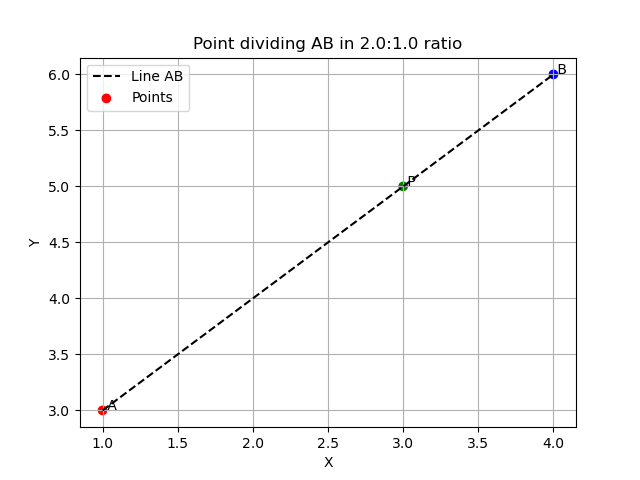
\includegraphics[width=\linewidth]{figs/q1.1.png}
	\end{center}
\end{frame}

\begin{frame}{Plot by python only}
	\begin{center}
		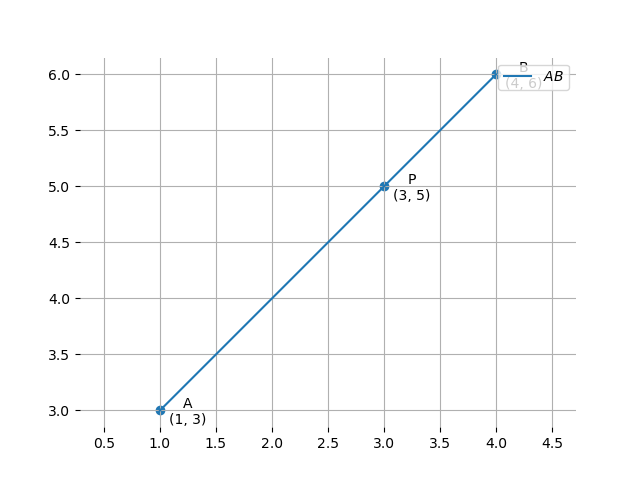
\includegraphics[width=\linewidth]{figs/q1.2.png}
	\end{center}
\end{frame}



\end{document}